\chapter{Рекомендательная система (ЛР3)}

\section{Постановка задачи и выбор подхода}

Рекомендательная система по профилю предпочтений пользователя строит ранжированный список объектов каталога. Разработаны три версии.
\begin{itemize}[leftmargin=1.6\parindent, label*=---]
	\item \textbf{PCv1 (v1)}. На вход подаётся один объект-затравка, на выходе получается список, ранжированный по убыванию близости к затравке.
	\item \textbf{PCv2 (v2)}. На вход подаётся набор лайков, на выходе получается ранжированный список.
	\item \textbf{PCv3 (v3)}. На вход подаются лайки и дизлайки, на выходе получается ранжированный список.
\end{itemize}

Выбран \textbf{контентный} подход. В нём релевантность объекта определяется сходством его признаков с объектами, которые понравились пользователю~\cite{lops2011, pazzani2007}. Коллаборативная фильтрация отвергнута. Она требует матрицы оценок многих пользователей, а в учебной системе таких данных нет. Контентный подход обладает свойствами, важными для этой задачи.
\begin{itemize}[leftmargin=1.6\parindent, label*=---]
	\item \textbf{Нет проблемы холодного старта для объектов.} Новый ликёр рекомендуется сразу после добавления в каталог, так как оценки других пользователей ему не нужны~\cite{schein2002}. Новому пользователю достаточно одного лайка. Это ровно режим v1.
	\item \textbf{Не возникает проблемы <<белой вороны>>.} Пользователю с редким вкусом не нужны похожие на него пользователи. Рекомендации строятся только по его собственному профилю.
	\item \textbf{Проблема устаревших предпочтений решается} учётом времени лайков в подходе Б и возможностью начать профиль заново.
\end{itemize}
Ограничение подхода --- узкая специализация. Система рекомендует только похожее на уже оценённое. Его частично компенсирует учёт нескольких групп интересов из раздела~\ref{sec:lr3_v2}.

\textbf{Как формируется ранжированный список.} Каждому кандидату $x$, то есть объекту каталога без оценки пользователя, сопоставляется числовая оценка релевантности $r(x)$. Список --- это кандидаты по убыванию $r(x)$. При равенстве они упорядочены по идентификатору, чтобы порядок был детерминированным. Пользователю показываются первые $N$ элементов. Все версии используют одну и ту же обобщающую меру близости из ЛР2~\eqref{eq:lr2_total}. Они различаются только способом вычисления $r(x)$. Попарные близости предвычисляются в матрицу $30\times30$. При таком размере каталога пересчёт не нужен, а доступ занимает $O(1)$.

\section{PCv1: рекомендации по затравке}

Для затравки $s$ релевантность равна близости к ней, то есть $r(x) = \mathrm{sim}(s, x)$. Затравка из выдачи исключается. Пример выдачи для двух затравок приведён в таблице~\ref{tab:lr3_v1}. В обоих случаях первые позиции занимают объекты того же листа или той же группы L2 таксономии.

\begin{table}[H]
	\centering
	\caption{Выдача PCv1, top-5}
	\label{tab:lr3_v1}
	\footnotesize
	\begin{tabular}{|L{3.2cm}|L{11.8cm}|}
		\hline
		Затравка & Выдача и релевантность \\ \hline
		L26 Cr\`eme de Cacao Brown & L27 Cacao White (0,883), L01 Cr\`eme de Menthe (0,647), L25 Kahl\'ua (0,632), L19 Cr\`eme de Banane (0,620), L12 Cr\`eme de Cassis (0,532) \\ \hline
		L05 Amaro Averna & L07 Montenegro (0,848), L06 Fernet-Branca (0,750), L03 J\"agermeister (0,618), L04 Chartreuse Verte (0,562), L23 Nocino (0,530) \\ \hline
	\end{tabular}
\end{table}

\section{PCv2: набор лайков}
\label{sec:lr3_v2}

\subsection{Рассмотренные подходы}

Пусть $L = (l_1,\ldots,l_m)$ --- лайки в порядке их установки, а $s_i(x) = \mathrm{sim}(x, l_i)$. Реализованы и сравнены шесть способов получить из нескольких лайков одну оценку или один список.

\textbf{А. Среднее арифметическое} считает $r(x) = \frac1m\sum_i s_i(x)$. Подход прост, но зависит от домена. Если лайки близки друг к другу, среднее работает как близость к центру интереса. Если пользователю нравятся два далёких объекта, среднее поднимает объекты посередине, не похожие ни на один из лайков. Например, при лайках Amaro Averna и Baileys в первую пятёрку попадает Ponche Crema. Шестым идёт Grand Marnier, близость которого к обоим лайкам около 0,4.

\textbf{Б. Учёт времени лайков} --- взвешенное среднее с весами $w_i = \gamma^{\,m-i}$, где $\gamma = 0{,}7$. Последний лайк весит 1, предыдущий 0,7 и так далее. Подход отражает смещение вкуса со временем и решает проблему устаревших предпочтений. Однако он наследует от А эффект <<середины>>.

\textbf{В. Взвешенное суммирование} задаёт веса не временем, а структурой профиля. Вес равен $w_i = 1/|G(l_i)|$, где $G(l_i)$ --- группа интересов лайка из подхода Г. Каждая группа интересов вносит одинаковый вклад, даже если в ней пять лайков, а в другой один.

\textbf{Максимум} считает $r(x) = \max_i s_i(x)$ как близость к ближайшему лайку. Эффекта <<середины>> нет, но одна группа интересов может занять всю выдачу.

\textbf{Г$'$. Сшивание списков по каждому лайку} строит для каждого лайка свой список по убыванию $s_i(x)$. Затем списки сшиваются по одному объекту от каждого по очереди, а дубликаты устраняются.

\textbf{Г. Выделение групп лайков} разбивает лайки на группы интересов. Две группы объединяются, если между какими-то их лайками близость не ниже порога $\theta$. Это компоненты связности графа лайков по одиночной связи. Внутри группы $g$ оценка равна среднему $r_g(x) = \frac1{|g|}\sum_{l\in g}\mathrm{sim}(x,l)$. Внутри связной группы эффекта <<середины>> нет, потому что середина между похожими объектами сама похожа на них. Итоговая выдача сшивается из списков групп по одному объекту от каждой группы без дубликатов. Группы упорядочены по размеру, и первой идёт группа с наибольшим числом лайков.

\subsection{Сравнение качества подходов}

Чтобы выбрать подход, нужна проверка, а не только рассуждение. Вкус пользователя смоделирован группами L2 таксономии~\cite{herlocker2004}. Пользователь с $k$ интересами лайкает все объекты $k$ групп L2, кроме последнего в каждой группе. Отложенные объекты нужно вернуть в top-5. Перебраны все сочетания групп. Получилось 12 сценариев при $k=1$, 66 при $k=2$ и 220 при $k=3$. Использованы три метрики.
\begin{itemize}[leftmargin=1.6\parindent, label*=---]
	\item \textbf{recall(5)} --- доля отложенных объектов в первых пяти позициях.
	\item \textbf{coverage(5)} --- доля групп интересов, которым служит хотя бы один элемент выдачи. Ближайший к элементу лайк лежит в этой группе. Метрика отражает разнообразие выдачи по интересам~\cite{ziegler2005}.
	\item \textbf{support(5)} --- средняя близость элемента выдачи к ближайшему лайку. Малое значение означает рекомендации, не похожие ни на что.
\end{itemize}

\begin{table}[H]
	\centering
	\caption{Сравнение подходов PCv2 при $N=5$. R --- recall(5), C --- coverage(5), S --- support(5)}
	\label{tab:lr3_v2_eval}
	\footnotesize\setlength{\tabcolsep}{4pt}
	\begin{tabular}{|l|c|c|c|c|c|c|}
		\hline
		& \multicolumn{3}{c|}{2 группы интересов (66)} & \multicolumn{3}{c|}{3 группы интересов (220)} \\ \cline{2-7}
		Подход & R & C & S & R & C & S \\ \hline
		А. среднее & 0,750 & 0,894 & 0,650 & 0,649 & 0,742 & 0,677 \\ \hline
		Б. время & 0,826 & 0,932 & 0,654 & 0,733 & 0,808 & 0,681 \\ \hline
		В. баланс групп & 0,818 & 0,955 & 0,659 & 0,747 & 0,836 & 0,691 \\ \hline
		максимум & 0,826 & 0,932 & 0,670 & 0,782 & 0,886 & 0,707 \\ \hline
		Г$'$. по каждому лайку & 0,818 & 1,000 & 0,657 & 0,796 & 0,983 & 0,690 \\ \hline
		\textbf{Г. группы лайков} & 0,811 & \textbf{1,000} & 0,658 & \textbf{0,797} & \textbf{1,000} & 0,693 \\ \hline
	\end{tabular}
\end{table}

\begin{figure}[H]
	\centering
	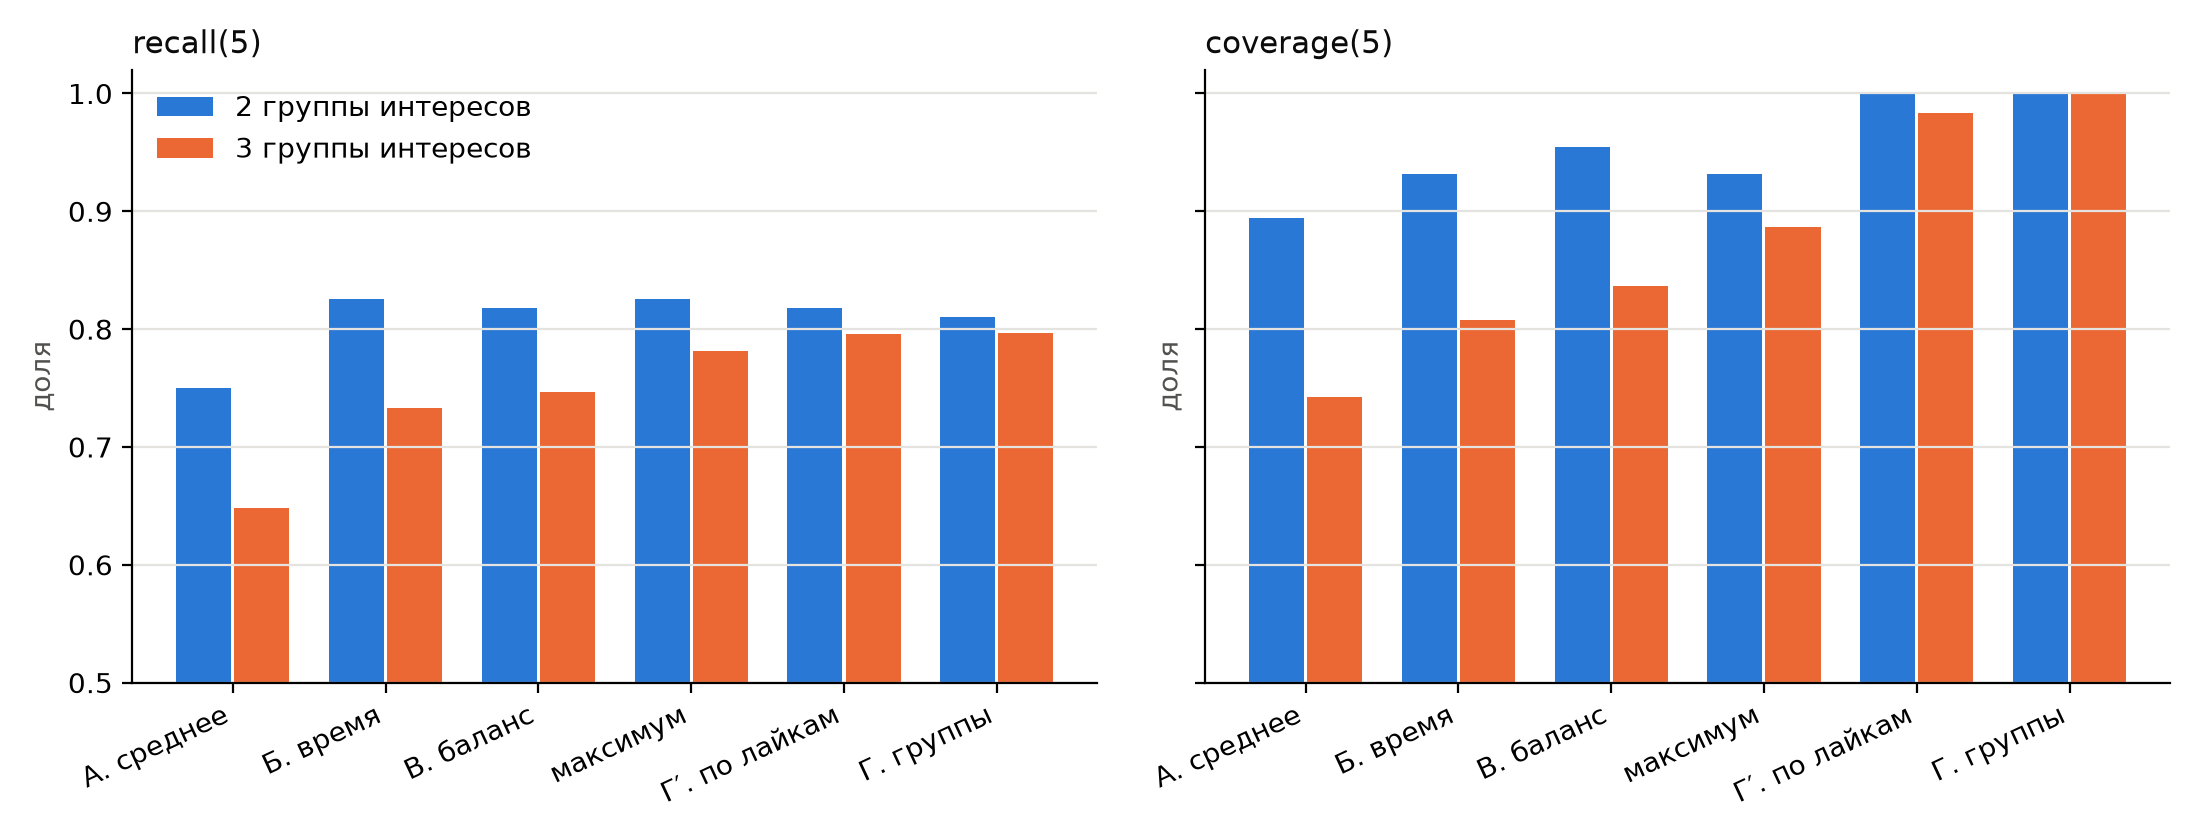
\includegraphics[width=\textwidth]{lr3/v2_rankers.png}
	\caption{Метрики recall(5) и coverage(5) подходов PCv2 для двух и трёх групп интересов}
	\label{fig:lr3_v2}
\end{figure}

При одной группе интересов все подходы равны и дают recall 0,917 и coverage 1. Различия появляются при нескольких интересах, что видно из таблицы~\ref{tab:lr3_v2_eval} и рисунка~\ref{fig:lr3_v2}. Среднее А оказалось хуже всех. При трёх интересах теряется треть отложенных объектов, а каждая четвёртая группа не представлена в выдаче. Учёт времени Б и баланс групп В улучшают среднее, но сохраняют его главный недостаток. Максимум даёт наибольший support. Каждый элемент его выдачи действительно близок к какому-то лайку, но не все интересы попадают в выдачу, coverage равен 0,886. Сшивание по лайкам Г$'$ и по группам Г обслуживают все интересы. При этом Г не даёт интересу с большим числом лайков занять несколько очередей сшивания. Три амаро и Baileys дают две группы, а не четыре списка. При двух интересах подходы Б, максимум, Г$'$ и Г различаются не более чем на один отложенный объект из 132. При трёх лучшим по recall и coverage оказывается Г.

\textbf{Выбор порога $\theta$.} Порог должен объединять лайки одного интереса и не склеивать разные. На рисунке~\ref{fig:lr3_relations} показано распределение итоговой близости пар по положению в таксономии. Пары из разных ветвей L1 не превышают 0,647, а медиана пар с общим L2 равна 0,667. Порог $\theta = 0{,}65$ лежит на этой границе. Перебор порога на рисунке~\ref{fig:lr3_theta} подтверждает выбор. При $\theta = 0{,}65$ достигается максимум recall(5) для трёх интересов, 0,797, и полное покрытие интересов. При меньших порогах разные интересы склеиваются, и coverage падает до 0,83.

\begin{figure}[H]
	\centering
	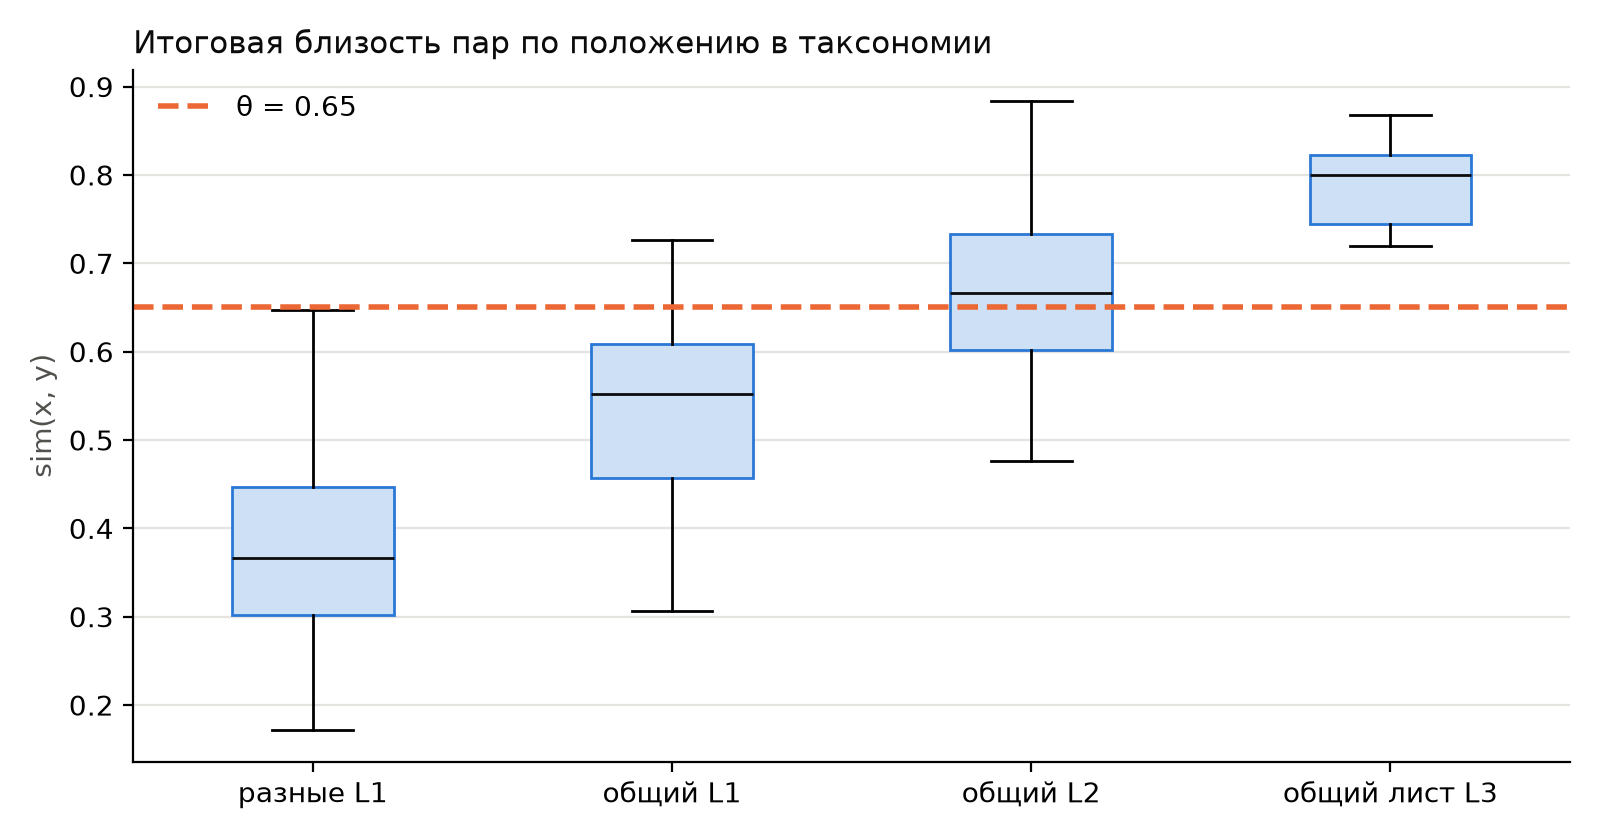
\includegraphics[width=0.82\textwidth]{lr3/sim_by_relation.png}
	\caption{Итоговая близость пар в зависимости от глубины общего предка в таксономии}
	\label{fig:lr3_relations}
\end{figure}

\begin{figure}[H]
	\centering
	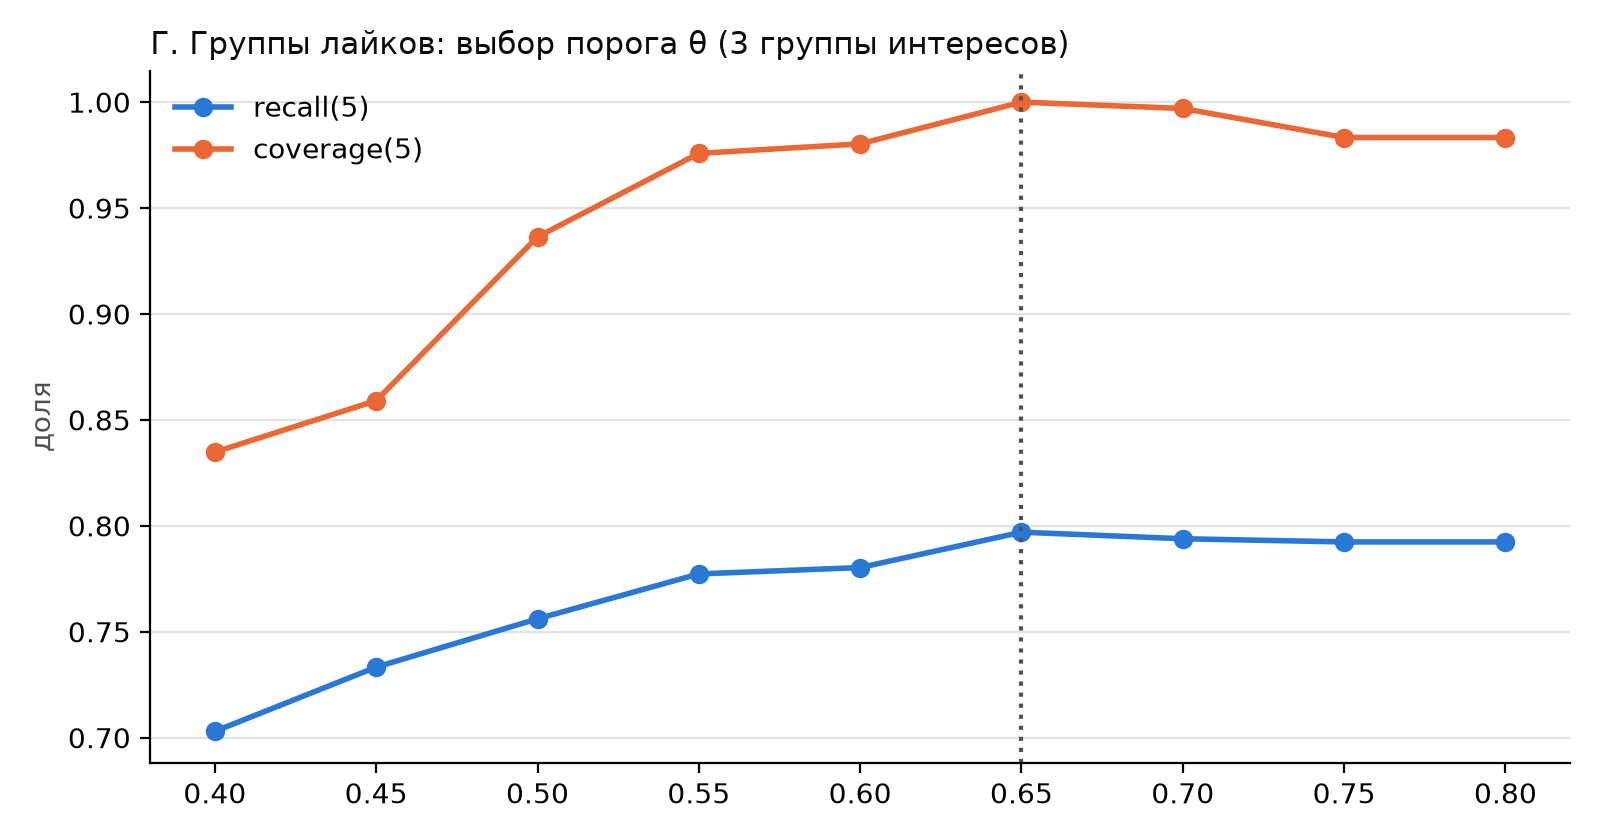
\includegraphics[width=0.82\textwidth]{lr3/v2_threshold.png}
	\caption{Подбор порога группировки $\theta$. Три группы интересов, 220 сценариев}
	\label{fig:lr3_theta}
\end{figure}

Пример выдачи для лайков <<Amaro Averna, Baileys>> в таблице~\ref{tab:lr3_v2_example} иллюстрирует разницу. Среднее занижает оценки и поднимает объекты между интересами. Максимум отдаёт четыре места из пяти амаро. Подход Г чередует интересы.

\begin{table}[H]
	\centering
	\caption{Выдача PCv2 для лайков L05 Amaro Averna и L28 Baileys}
	\label{tab:lr3_v2_example}
	\footnotesize
	\begin{tabular}{|L{3.4cm}|L{11.6cm}|}
		\hline
		Подход & top-5 и оценка \\ \hline
		А. среднее & L07 (0,571), L29 (0,557), L06 (0,478), L03 (0,423), L13 (0,420) \\ \hline
		Б. время & L29 (0,581), L07 (0,522), L13 (0,435), L06 (0,430), L10 Grand Marnier (0,414) \\ \hline
		максимум & L07 (0,848), L06 (0,750), L29 (0,696), L03 (0,618), L04 (0,562) \\ \hline
		Г. группы лайков & L07 (0,848), L29 (0,696), L06 (0,750), L13 (0,504), L03 (0,618) \\ \hline
	\end{tabular}
\end{table}

\textbf{Итог PCv2. По умолчанию используется подход Г} с порогом $\theta = 0{,}65$. Остальные подходы доступны в интерфейсе для сравнения. Выбор подтверждён проверкой на датасете. Он согласуется с идеей выделения групп лайков, где одну группу можно усреднять, а разные группы нужно показывать по очереди.

\section{PCv3: лайки и дизлайки}

\subsection{Рассмотренные подходы}

Дизлайк несёт информацию, противоположную лайку. Однако использовать её симметрично нельзя. Типичная ситуация взята из примера с музыкой. Пользователю нравится весь жанр и почти весь материал исполнителя, кроме одной композиции. Если штрафовать всё, что похоже на эту композицию, система испортит весь любимый жанр. Дизлайк должен сужать интерес, а не отменять его. Анкетирование о причинах неприязни отвергнуто. Длинная анкета раздражает пользователя, и он может уйти. Причину неприязни система должна вывести из соотношения лайков и дизлайков. Реализованы четыре политики учёта дизлайков $D$. Через $\mathrm{dis}(x) = \max_{d\in D}\mathrm{sim}(x,d)$ обозначена близость к ближайшему дизлайку, а через $\mathrm{sup}(x) = \max_{l\in L}\mathrm{sim}(x,l)$ --- к ближайшему лайку.
\begin{enumerate}[leftmargin=1.6\parindent]
	\item \textbf{Только исключить дизлайки.} Из выдачи убираются сами дизлайкнутые объекты, остальное не меняется.
	\item \textbf{Исключить похожие.} Объект $x$ убирается, если $\mathrm{dis}(x)\geq\tau$, где $\tau = 0{,}7$.
	\item \textbf{Вычитание} по аналогии с формулой Роккио~\cite{rocchio1971, manning2008}, то есть $r'(x) = r(x) - \beta\,\mathrm{dis}(x)$.
	\item \textbf{Контрастный штраф} $r'(x) = r(x) - \beta\max\bigl(0,\ \mathrm{dis}(x) - \mathrm{sup}(x)\bigr)$. Штрафуется только то, что ближе к дизлайку, чем к любому лайку. Объекты любимого жанра близки и к дизлайку, и к лайкам того же жанра. Поэтому они почти не штрафуются, а объекты, похожие именно на нелюбимый образец, опускаются.
\end{enumerate}
Если у пользователя есть только дизлайки, оценка равна $r(x) = 1 - \mathrm{dis}(x)$. Рекомендуется то, что дальше всего от нелюбимого.

\subsection{Сравнение качества политик}

Два протокола моделируют два требования.
\begin{itemize}[leftmargin=1.6\parindent, label*=---]
	\item \textbf{Дизлайк внутри любимого жанра}, 38 сценариев. В группе L2 из трёх и более объектов один объект дизлайкнут, один отложен, остальные лайкнуты. Хорошая политика сохраняет жанр, и recall отложенного объекта остаётся высоким.
	\item \textbf{Дизлайк чужого жанра}, 132 сценария. Лайки из группы A, дизлайк --- один объект группы B. Хорошая политика не рекомендует остальные объекты группы B. Мера leakage(5), доля таких объектов в выдаче, должна быть низкой, а recall отложенного объекта из A --- высоким.
\end{itemize}

\begin{table}[H]
	\centering
	\caption{Сравнение политик учёта дизлайков. Стратегия лайков Г, $N=5$}
	\label{tab:lr3_v3_eval}
	\footnotesize
	\begin{tabular}{|L{5.6cm}|L{2.6cm}|L{2.6cm}|L{2.6cm}|}
		\hline
		Политика и параметр & recall, свой жанр & recall, чужой жанр & leakage, чужой жанр \\ \hline
		1. только исключить & 0,974 & 0,917 & 0,049 \\ \hline
		2. исключить похожие, $\tau=0{,}7$ & 0,447 & 0,924 & 0,029 \\ \hline
		2. исключить похожие, $\tau=0{,}8$ & 0,763 & 0,932 & 0,039 \\ \hline
		3. вычитание, $\beta=1$ & 0,368 & 0,902 & 0,002 \\ \hline
		3. вычитание, $\beta=0{,}25$ & 0,921 & 0,939 & 0,023 \\ \hline
		4. контрастный, $\beta=0{,}5$ & 0,947 & 0,932 & 0,026 \\ \hline
		\textbf{4. контрастный, $\beta=1$} & \textbf{0,921} & \textbf{0,932} & \textbf{0,017} \\ \hline
		4. контрастный, $\beta=2$ & 0,842 & 0,917 & 0,012 \\ \hline
	\end{tabular}
\end{table}

\begin{figure}[H]
	\centering
	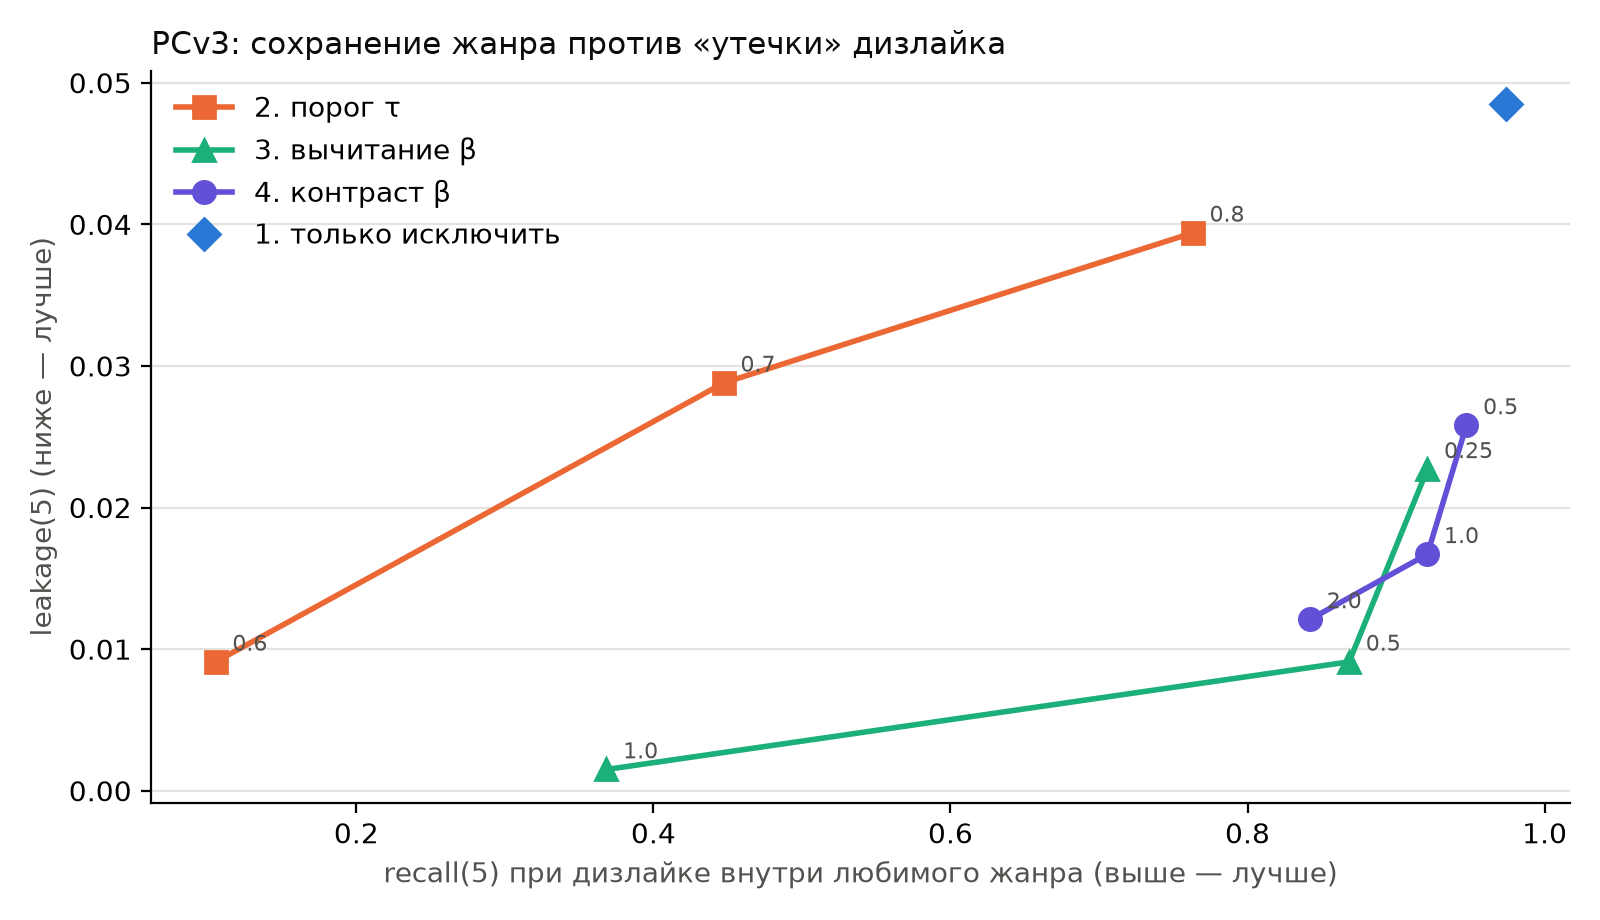
\includegraphics[width=0.85\textwidth]{lr3/v3_tradeoff.png}
	\caption{Компромисс <<сохранение жанра и утечка дизлайка>>. Подписи точек --- значения $\tau$ или $\beta$}
	\label{fig:lr3_v3}
\end{figure}

Результаты приведены в таблице~\ref{tab:lr3_v3_eval} и на рисунке~\ref{fig:lr3_v3}.
\begin{itemize}[leftmargin=1.6\parindent, label*=---]
	\item политика 1 лучше всех сохраняет жанр, но почти не реагирует на дизлайк. Утечка у неё самая большая, 0,049.
	\item исключение по порогу и вычитание с полной силой $\beta=1$ портят жанр. Recall в своём жанре падает до 0,37--0,45. Так проявляется проблема из примера с музыкой.
	\item вычитание с малым $\beta=0{,}25$ сохраняет жанр, но примерно в 1,4 раза хуже по утечке, чем контрастный штраф с $\beta=1$.
	\item \textbf{контрастный штраф с $\beta=1$} --- лучший компромисс. Утечка втрое ниже, чем у политики 1, при почти той же сохранности жанра 0,921 и лучшем recall в чужом жанре 0,932.
\end{itemize}

Таблица~\ref{tab:lr3_v3_example} показывает это на примерах. В первом пользователь любит травяные ликёры J\"agermeister, Averna и Montenegro, но не любит Fernet-Branca. Вычитание выдаёт сливочные ликёры с оценками около 0,1, то есть жанр потерян. Контрастный штраф оставляет Chartreuse и G\'en\'epi. Во втором примере Baileys нравится, а яичный Advocaat нет. Контрастный штраф опускает яичный Ponche Crema со второго места на пятое со штрафом 0,223. Причина в том, что он ближе к Advocaat, 0,727, чем к Baileys, 0,504.

\begin{table}[H]
	\centering
	\caption{Выдача PCv3 при разных политиках учёта дизлайков}
	\label{tab:lr3_v3_example}
	\footnotesize
	\begin{tabular}{|L{2.7cm}|L{6cm}|L{6cm}|}
		\hline
		Политика & лайки L03, L05, L07 и дизлайк L06 & лайк L28 и дизлайк L30 \\ \hline
		1. исключить & L04, L02, L24, L23, L22 & L29, L13, L10, L22, L05 \\ \hline
		2. порог $\tau$ & L04, L02, L24, L23, L22 & L29, L10, L22, L05, L11 \\ \hline
		3. вычитание & L29, L28, L14, L25, L18, оценки 0,07--0,11 & L29, L10, L05, L23, L06 \\ \hline
		\textbf{4. контрастный} & L04, L02, L24, L23, L22 & L29, L10, L05, L23, L13 \\ \hline
	\end{tabular}
\end{table}

\textbf{Итог PCv3. Используется контрастный штраф с $\beta = 1$.} Он формализует интуицию <<дизлайк уточняет, а не отменяет интерес>> и подтверждён проверкой на датасете.

\section{Объяснение рекомендаций}

Пользователь должен понимать, почему ему рекомендован объект. Для каждого элемента выдачи система сохраняет ближайший лайк вроде <<похож на Baileys>>, номер группы интересов и вклад каждой частной меры $\omega_k\,\mathrm{sim}_k$ в близость к этому лайку. Если сработал штраф, показываются его размер и дизлайк, на который похож объект. Объяснение стоит дёшево. Обобщающая мера~\eqref{eq:lr2_total} аддитивна, и её слагаемые уже вычислены.

\section{Пользовательский интерфейс}

На рисунке~\ref{fig:ui_lr3_v1} показан режим PCv1. Слева каталог с карточками ликёров, справа профиль и выдача с оценкой и объяснением.

\begin{figure}[H]
	\centering
	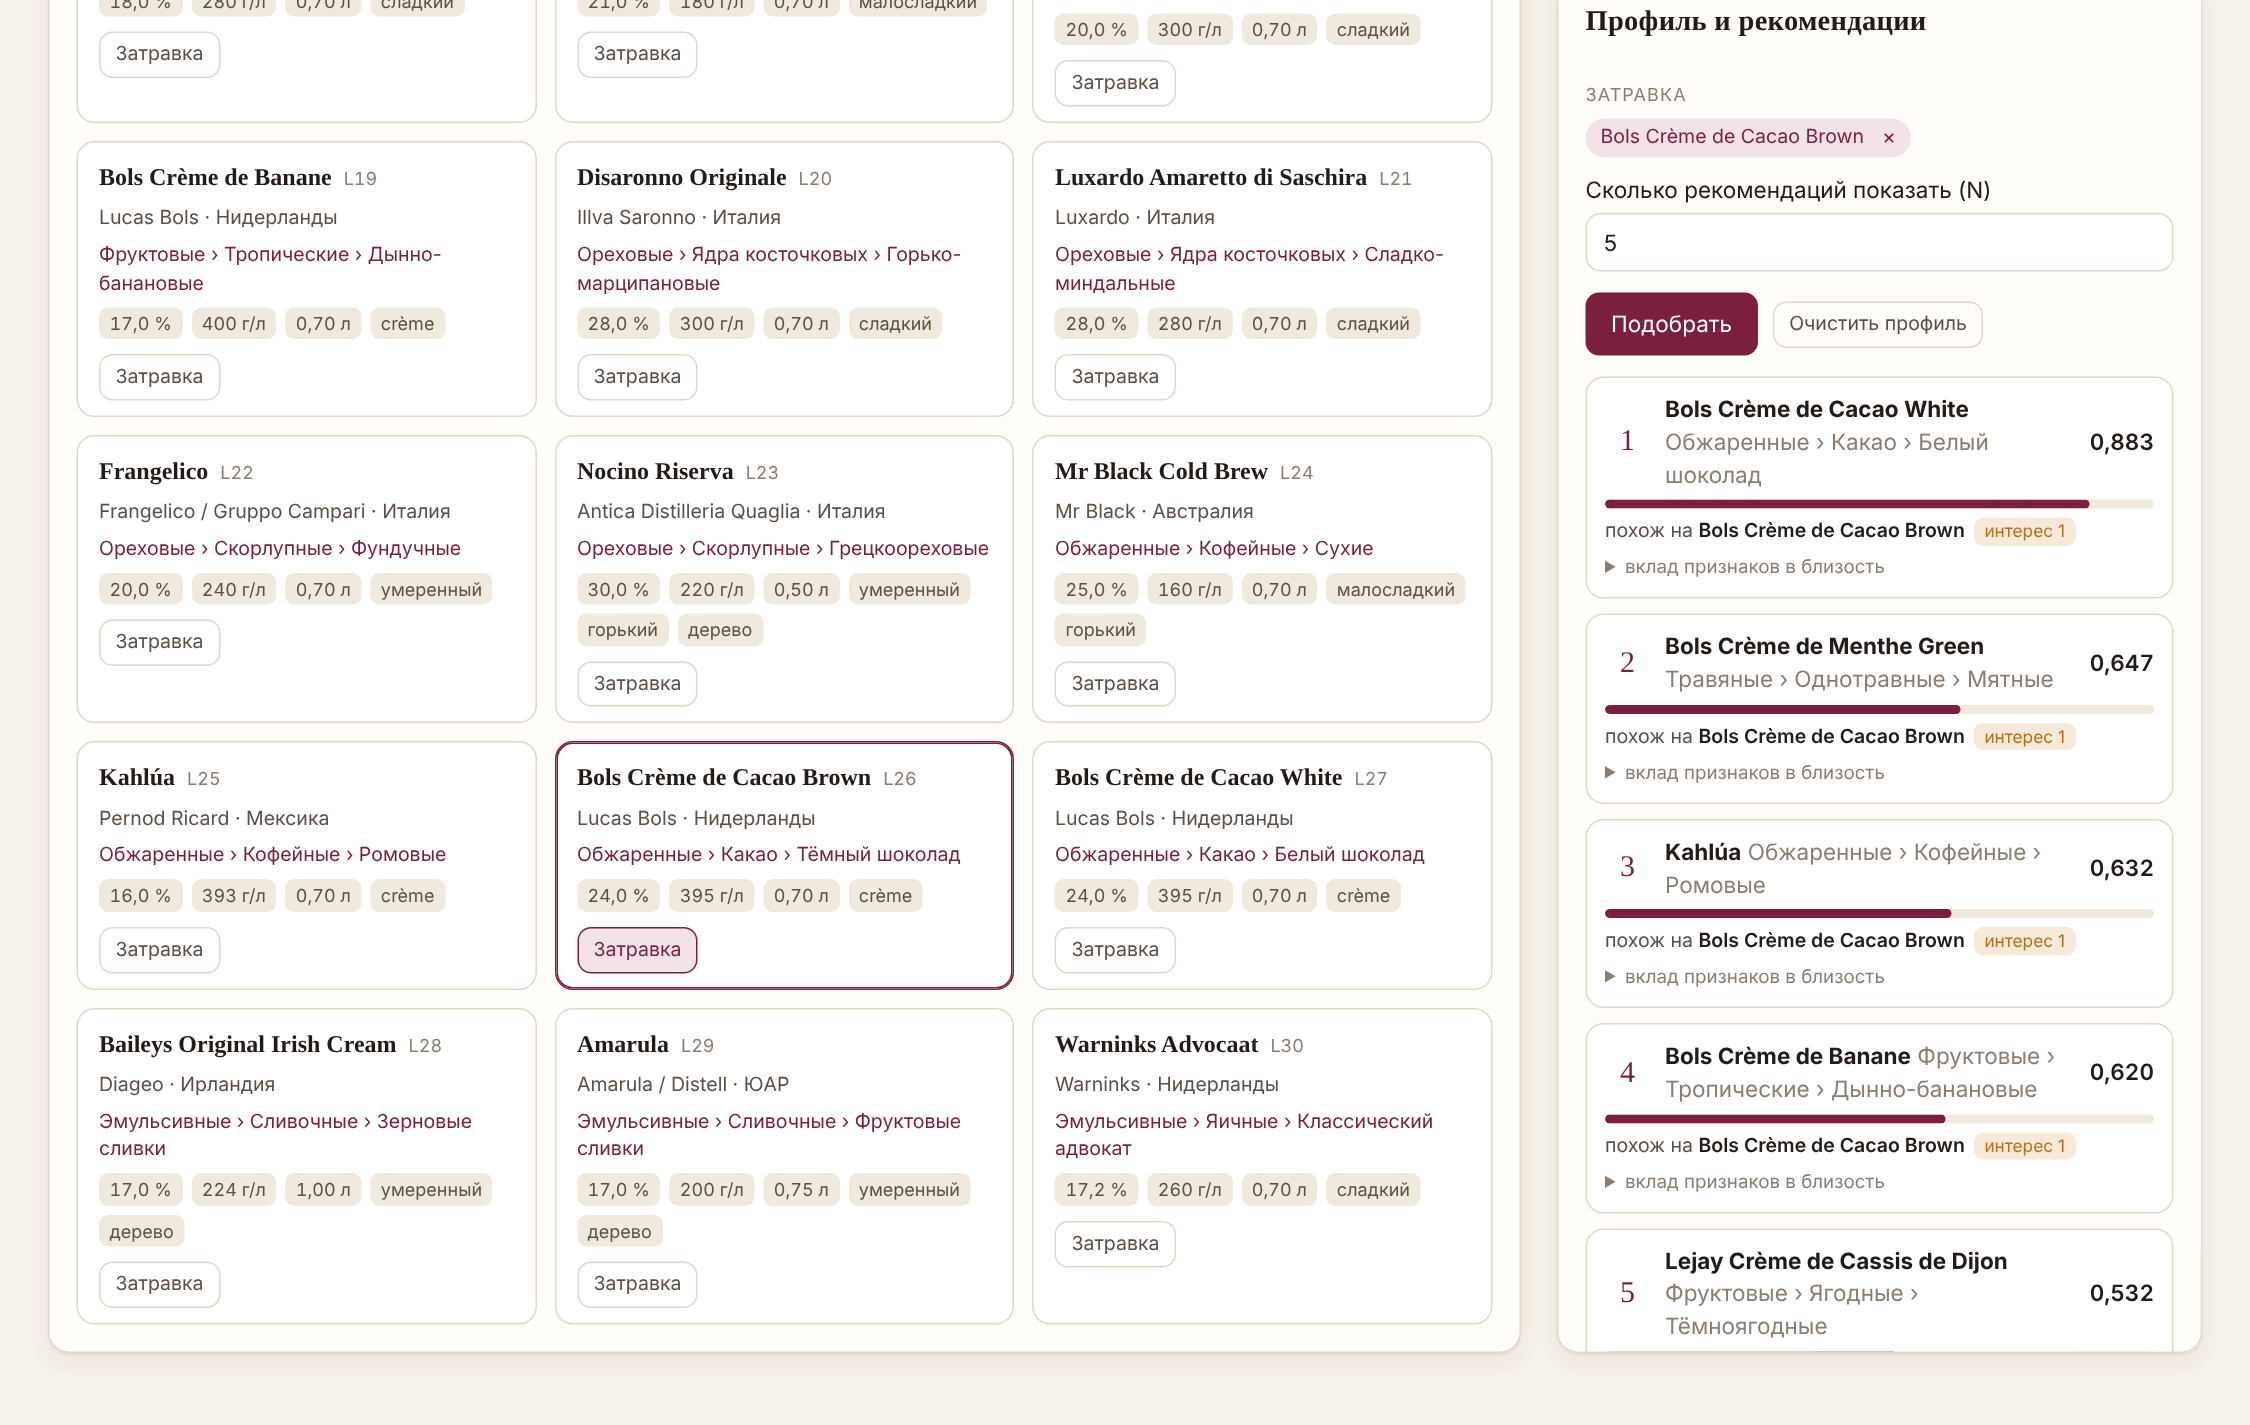
\includegraphics[width=\textwidth]{ui/lr3_v1.png}
	\caption{PCv1. Затравка Cr\`eme de Cacao Brown}
	\label{fig:ui_lr3_v1}
\end{figure}

На рисунке~\ref{fig:ui_lr3_v3} показаны режимы PCv2 и PCv3. В первом пользователь ставит несколько лайков, и выдача чередует группы интересов. Во втором добавляются дизлайки, и у наказанных объектов видны штраф и его причина.

\begin{figure}[H]
	\centering
	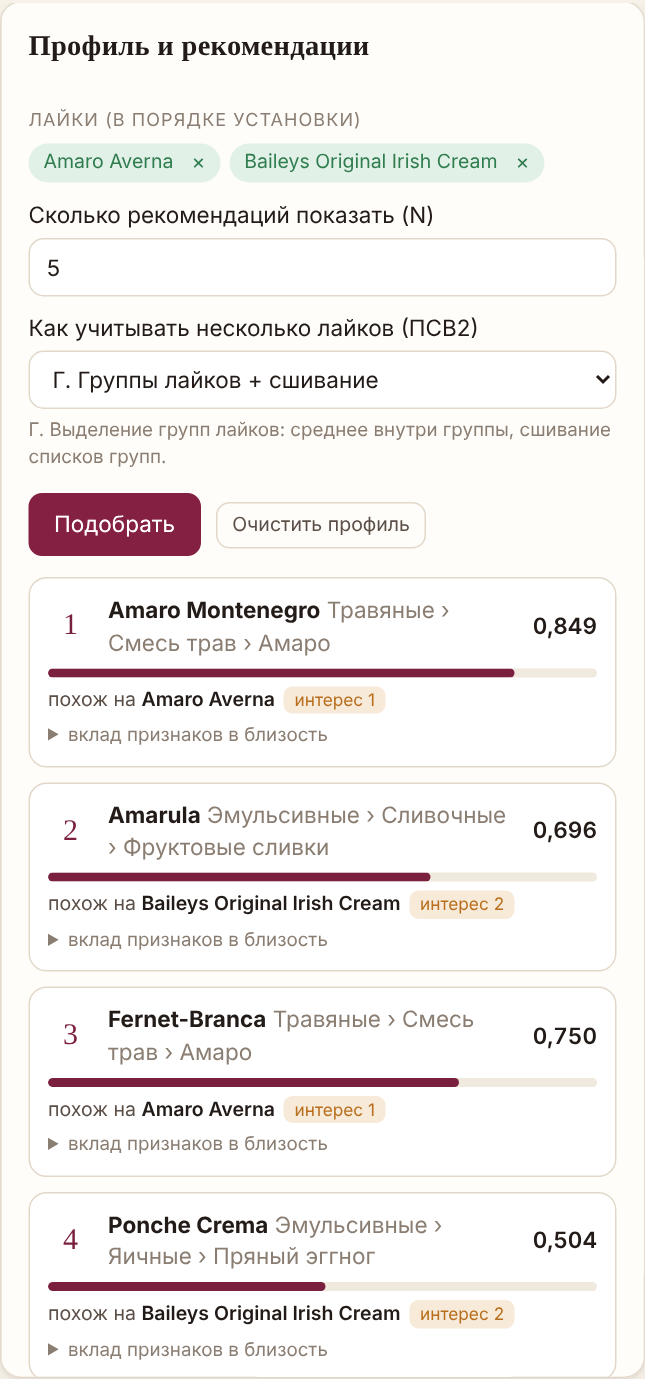
\includegraphics[width=0.48\textwidth]{ui/lr3_v2_panel.png}\hfill
	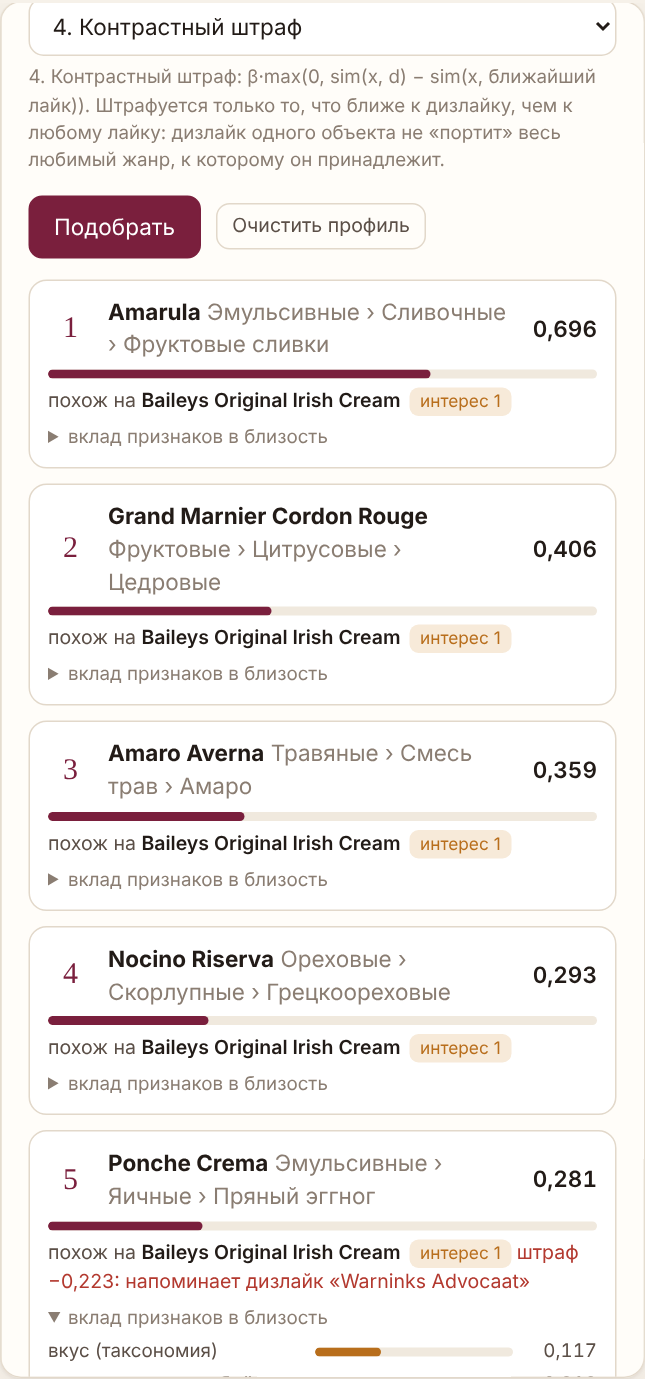
\includegraphics[width=0.48\textwidth]{ui/lr3_v3_panel.png}
	\caption{PCv2. Лайки Averna и Baileys с чередованием групп интересов слева. PCv3. Лайк Baileys и дизлайк Advocaat, штраф Ponche Crema с вкладом признаков справа}
	\label{fig:ui_lr3_v3}
\end{figure}

Ввод проверяется на сервере, и все ошибки возвращаются одним списком. Пример такого списка показан на рисунке~\ref{fig:ui_lr3_errors}.

\begin{figure}[H]
	\centering
	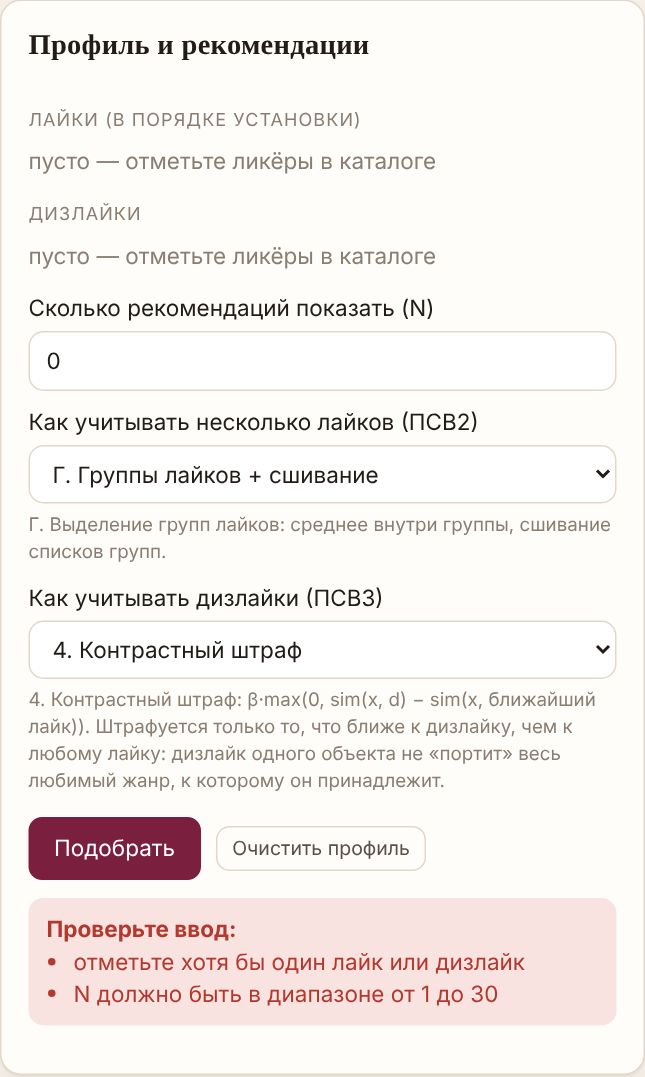
\includegraphics[width=0.48\textwidth]{ui/lr3_errors.png}
	\caption{Сообщения об ошибках ввода для пустого профиля и $N = 0$}
	\label{fig:ui_lr3_errors}
\end{figure}

\section*{Выводы}
\addcontentsline{toc}{section}{Выводы}

Разработана контентная рекомендательная система в трёх версиях с веб-интерфейсом. Для PCv2 сравнены шесть подходов и выбран подход Г <<группы лайков со сшиванием>> с порогом $\theta = 0{,}65$. При трёх интересах он даёт наибольшие recall(5), 0,797, и coverage(5), 1,0. Для PCv3 сравнены четыре политики учёта дизлайков и выбран контрастный штраф с $\beta = 1$. Он втрое снижает утечку нелюбимого стиля и почти не портит любимый жанр. Каждая рекомендация сопровождается объяснением. Рекомендательное ядро использовано в ЛР4 без изменений.
